\section{Conclusión y trabajo futuro}

\begin{frame}{Herramientas}
%Herramientas utilizadas en \textit{FuDePAN}:\\[0.3cm]
\begin{itemize}
\item Google Code (svn, issue tracking, reviews, wiki, etc.).
\item Toolchain de GNU.
\begin{itemize}
    \item g++
    \begin{itemize}
    \item -Wall
    \item -pedantic
    \item -ansi
    \item -Weffc++
    \end{itemize}
    \item gdb
    \item gcov
\end{itemize}
\item CCCC
\item CLOC
\item gprof (GNU Profiler).
\item Valgrind
\item astyle (Artistic Style).
\item Doxygen
\item CMake
\end{itemize}

\end{frame}


\subsection{Conclusión}

\begin{frame}{Conclusión}

    \begin{itemize}
     \item \rc\ funciona correctamente, independientemente del problema a resolver
     \item Nueva version de \fud\ funcional compatible hacia atrás que funciona con la misma eficacia que antes.
     \item Se abordaron técnicas y conceptos no vistos a lo largo de la carrera.
     \item Se obtuvo un experiencia de desarrolo satisfactoria trabajando en conjunto con otros grupos, local y remotamente.
    \end{itemize}

\end{frame}


\subsection{Trabajo futuro}

\begin{frame}{Trabajo futuro}

    \begin{itemize}
        \item Proveer de nuevas políticas de distribución concretas.
        \item Adaptar esta capa para que proyectos \textbf{\textit{BOINC}} funcionen sobre ella.
        \item Correr \textit{\textbf{RNAFEE}} en ``modo completo'' en un cluster
        \item Reimplementar sobre \rc\ el generador de cadenas de proteínas \textit{backbones-generator}
    \end{itemize}
\end{frame}


\begin{frame}{Backbones Generator}
    
    Es un proyecto que tiene como objetivo construir una base de datos de las posibles cadenas principales (backbones) de
    proteínas.\\[0.5cm]
    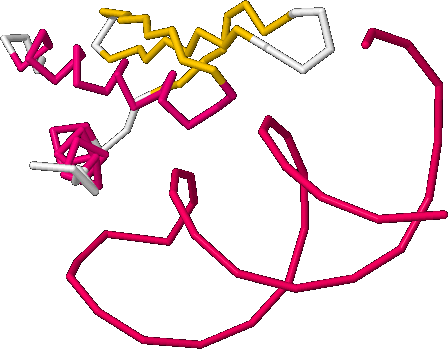
\includegraphics[height=120pt]{images/2L3C-backbone.png} 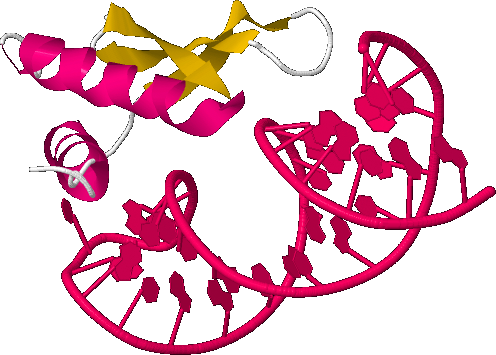
\includegraphics[height=120pt]{images/2L3C-cartoon.png}\\[0.2cm]
    \qquad \qquad \qquad \textit{backbone} \qquad \qquad \qquad \qquad \qquad \textit{proteína específica}
\end{frame}

\begin{frame}{Backbones Generator}
    \textit{Características:}
    \begin{itemize}
        \item Una predicción de una proteína puede durar varios meses.
        \item Una proteína tiene dos partes: cadena principal y cadenas laterales que la diferencian.
    \end{itemize}
    \begin{center}
        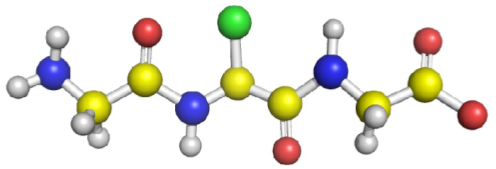
\includegraphics[height=40pt]{images/backbone.png}
    \end{center}
    \pause
    \begin{block}{Idea}
        Hacer por \textbf{única vez} un cálculo gigante que arroje una base de datos de todos los esqueletos de proteínas posibles de
        tamaño máximo dado.
    \end{block}
\end{frame}


%%%%%%%%%%%%%%%% BIBLIOGRAFIA %%%%%%%%%%%%%%%%
\nocite{alsuwaiyel98}
\nocite{bellman10}
\nocite{clus09}
\nocite{uml}
\nocite{buyya99}
\nocite{cormen09}
\nocite{ewd1036}
\nocite{algorithms06}
\nocite{flynn}
\nocite{parallel}
\nocite{conmath94}
\nocite{levitin06}
\nocite{Liskov:1987:KAD:62139.62141}
\nocite{Lorin:1990:RHP:1011116.1011127}
\nocite{objmentor}
\nocite{martin-asd}
\nocite{oosc}
\nocite{pressman}
\nocite{svn}
\nocite{sigler03}
\nocite{skiena08}
\nocite{moshe10}
\nocite{cplusplus}
\nocite{algdatpro76}

\begin{frame}[allowframebreaks]{Bibliografía} 
    \bibliography{biblio}
    \bibliographystyle{annotate}
\end{frame}

%%%%%%%%%%%%%%%% PREGUNTAS %%%%%%%%%%%%%%%%
\begin{frame}
    \centerline{\Huge{\textbf{?`Preguntas?}}}
\end{frame}

%%%%%%%%%%%%%%%% GRACIAS %%%%%%%%%%%%%%%%
\begin{frame}
    \centerline{\Huge{\textbf{GRACIAS}}}
\end{frame}
